% Results (Task 42): three RQs; claims table of handoff/37_narrative_v2.md sections 3.3 and 3.7 applied; A6x answers
% the selection question. Every result number is a macro.
\section{Results}
\label{sec:results}

Unless stated otherwise, numbers in this section are V1 values (Section~\ref{sec:setup}) on the \nCommonClasses{}
common classes at $\epsilon = \paramEpsHead$, given as the mean over seeds with the seed range in brackets.
V1 is the primary row set; V0 and V2 are in Section~\ref{sec:rq3} and Appendices~\ref{sec:sens} and~\ref{sec:supp}.

\subsection{RQ1: attention is stable but not faithful}
\label{sec:rq1}
\emph{Answer: rollout attention agreed weakly to moderately with attribution methods and was less faithful than IG and
occlusion on both datasets; it changed little under constrained attacks that targeted it, and after an evasion its
faithfulness fell together with that of the other explanation methods.}

\paragraph{Clean data.}
Rollout attention agreed weakly to moderately with the attribution methods on both datasets: its Spearman correlation
was highest with GradientSHAP (\spRolloutGShapVoneSeventeen{} on 2017, \spRolloutGShapVoneEighteen{} on 2018), about one
third with IG (\spRolloutIGVoneSeventeen{}, range \spRolloutIGVoneSeventeenRange; \spRolloutIGVoneEighteen{}, range
\spRolloutIGVoneEighteenRange), \spRolloutOcclVoneSeventeen{} and \spRolloutOcclVoneEighteen{} with occlusion, and
lowest with TreeSHAP of the XGBoost model (\spRolloutTreeShapVoneSeventeen{} and \spRolloutTreeShapVoneEighteen;
Table~\ref{t_clean}).
Last-layer attention showed almost no agreement (Spearman with IG \spLastIGVoneSeventeen{} and \spLastIGVoneEighteen).
Rollout was more faithful than random and less faithful than IG and occlusion.
Its deletion AUC was \aucDelRolloutVoneSeventeen{} on 2017 and \aucDelRolloutVoneEighteen{} on 2018, against
\aucDelIGVoneSeventeen{} and \aucDelIGVoneEighteen{} for IG, \aucDelOcclVoneSeventeen{} and \aucDelOcclVoneEighteen{}
for occlusion, and \aucDelRandomVoneSeventeen{} and \aucDelRandomVoneEighteen{} for random, and insertion AUC gave the
same picture (Table~\ref{t_clean}).
Among the \nMethods{} methods, rollout ranked \rankDelRolloutSeventeen{} and \rankDelRolloutEighteen{} by deletion AUC,
and the ordering of the methods was similar across the datasets (Spearman correlation between the two orderings
\ordSpDelVone{} for deletion and \ordSpInsVone{} for insertion AUC).
Three smaller 2017 results that did not hold on 2018 and a parameter-randomisation check are in
Appendices~\ref{sec:supp} and~\ref{sec:rand}.

% Generated by paper_v3/gen/make_tables_v3.py on 2026-10-30. Do not edit.
% Source: results/stage8/clean_variants.csv
% Source: results/stage8/clean_variants_ordering.csv
\begin{table}[t]
\centering
\footnotesize
\caption{Clean data (V1, 7 common classes): agreement of attention with attribution methods, and deletion and insertion faithfulness of 8 explanation methods.}
\label{t_clean}
\sbox0{%
\begin{tabular}{lcccc}
\toprule
Quantity & 2017 & 2018 & Rank 2017 & Rank 2018 \\
\midrule
\multicolumn{5}{l}{\textit{Agreement: Spearman correlation between attention and attribution rankings}} \\
Attn. rollout vs IG & $0.349$ {\scriptsize ($0.317$ to $0.373$)} & $0.314$ {\scriptsize ($0.244$ to $0.406$)} &  &  \\
Attn. rollout vs GradientSHAP & $0.470$ {\scriptsize ($0.412$ to $0.505$)} & $0.432$ {\scriptsize ($0.365$ to $0.515$)} &  &  \\
Attn. rollout vs Occlusion & $0.396$ {\scriptsize ($0.351$ to $0.435$)} & $0.358$ {\scriptsize ($0.310$ to $0.429$)} &  &  \\
Attn. rollout vs TreeSHAP (XGB) & $0.231$ {\scriptsize ($0.176$ to $0.269$)} & $0.263$ {\scriptsize ($0.226$ to $0.337$)} &  &  \\
Attn. layer mean vs IG & $0.306$ {\scriptsize ($0.268$ to $0.340$)} & $0.238$ {\scriptsize ($0.190$ to $0.334$)} &  &  \\
Attn. last layer vs IG & $0.033$ {\scriptsize ($-0.013$ to $0.092$)} & $0.015$ {\scriptsize ($-0.015$ to $0.048$)} &  &  \\
\midrule
\multicolumn{5}{l}{\textit{Deletion AUC (train-mean masking; lower is more faithful; rank 1 = lowest)}} \\
Attn. rollout & $0.125$ {\scriptsize ($0.114$ to $0.137$)} & $0.119$ {\scriptsize ($0.084$ to $0.178$)} & $5$ & $4$ \\
Attn. layer mean & $0.145$ {\scriptsize ($0.111$ to $0.191$)} & $0.140$ {\scriptsize ($0.113$ to $0.193$)} & $6$ & $5$ \\
Attn. last layer & $0.241$ {\scriptsize ($0.219$ to $0.272$)} & $0.259$ {\scriptsize ($0.174$ to $0.338$)} & $7$ & $7$ \\
IG & $0.020$ {\scriptsize ($0.015$ to $0.024$)} & $0.031$ {\scriptsize ($0.025$ to $0.039$)} & $1$ & $1$ \\
GradientSHAP & $0.058$ {\scriptsize ($0.054$ to $0.061$)} & $0.053$ {\scriptsize ($0.044$ to $0.065$)} & $3$ & $3$ \\
Occlusion & $0.024$ {\scriptsize ($0.018$ to $0.032$)} & $0.049$ {\scriptsize ($0.032$ to $0.067$)} & $2$ & $2$ \\
$|x|$ & $0.079$ {\scriptsize ($0.074$ to $0.084$)} & $0.149$ {\scriptsize ($0.122$ to $0.173$)} & $4$ & $6$ \\
Random & $0.246$ {\scriptsize ($0.240$ to $0.258$)} & $0.345$ {\scriptsize ($0.323$ to $0.380$)} & $8$ & $8$ \\
\multicolumn{3}{l}{\textit{Spearman of the method ordering, 2017 vs 2018}} & \multicolumn{2}{c}{$0.929$} \\
\midrule
\multicolumn{5}{l}{\textit{Insertion AUC (train-mean masking; higher is more faithful; rank 1 = highest)}} \\
Attn. rollout & $0.501$ {\scriptsize ($0.460$ to $0.577$)} & $0.607$ {\scriptsize ($0.541$ to $0.687$)} & $5$ & $4$ \\
Attn. layer mean & $0.470$ {\scriptsize ($0.420$ to $0.544$)} & $0.506$ {\scriptsize ($0.378$ to $0.578$)} & $6$ & $6$ \\
Attn. last layer & $0.252$ {\scriptsize ($0.207$ to $0.285$)} & $0.374$ {\scriptsize ($0.328$ to $0.442$)} & $7$ & $7$ \\
IG & $0.761$ {\scriptsize ($0.736$ to $0.793$)} & $0.864$ {\scriptsize ($0.837$ to $0.878$)} & $1$ & $1$ \\
GradientSHAP & $0.584$ {\scriptsize ($0.578$ to $0.593$)} & $0.795$ {\scriptsize ($0.770$ to $0.817$)} & $4$ & $3$ \\
Occlusion & $0.717$ {\scriptsize ($0.680$ to $0.778$)} & $0.795$ {\scriptsize ($0.782$ to $0.812$)} & $2$ & $2$ \\
$|x|$ & $0.636$ {\scriptsize ($0.629$ to $0.649$)} & $0.604$ {\scriptsize ($0.560$ to $0.656$)} & $3$ & $5$ \\
Random & $0.246$ {\scriptsize ($0.239$ to $0.257$)} & $0.342$ {\scriptsize ($0.320$ to $0.379$)} & $8$ & $8$ \\
\multicolumn{3}{l}{\textit{Spearman of the method ordering, 2017 vs 2018}} & \multicolumn{2}{c}{$0.929$} \\
\bottomrule
\end{tabular}}%
\ifdim\wd0>\textwidth\resizebox{\textwidth}{!}{\usebox0}\else\usebox0\fi
\par\smallskip\parbox{\linewidth}{\scriptsize Macro over the 7 common attack classes, mean over 3 seeds (seed range in brackets), V1 (explanation rows without a near duplicate in the training set). Ranks: position among the 8 methods from the 7-class means. Agreement of the layer-mean and last-layer attention with the other attributions, and all explanation rows (V0): Appendix~\ref{sec:supp}.}
\end{table}


\paragraph{Attention under constrained attacks.}
Under the constrained attack A2, which kept the prediction and minimised the rollout attention on the clean
top-\paramTopK{} IG features, the attention mass on these features kept \massAtwoVoneSeventeen{}
(\massAtwoVoneSeventeenRange) of its clean value on 2017 and \massAtwoVoneEighteen{} (\massAtwoVoneEighteenRange) on
2018, a mean reduction of \massRedAtwoVoneSeventeen{} and \massRedAtwoVoneEighteen{} (Figure~\ref{f_mass_ratio},
Table~\ref{t_attn_attack}).
Under the random control A0 at the same budget the mass kept \massAzeroVoneSeventeen{} (\massAzeroVoneSeventeenRange)
on 2017 and \massAzeroVoneEighteen{} (\massAzeroVoneEighteenRange) on 2018; no comparison with IG at an equal budget
was run.
The joint attack A3 with $\lambda = 1000$ reached \massAthreeVoneSeventeen{} and \massAthreeVoneEighteen.
The unconstrained reference moved the mass further at a standardised budget of $\epsilon = 0.5$ (\massUncVoneSeventeen{}
and \massUncVoneEighteen, a reduction of \massRedUncVoneSeventeen{} and \massRedUncVoneEighteen), with rows that are not
valid flows and with a budget that is not in the units of the constrained attacks.
Attention was therefore stiff under the feature constraints; this does not show that attention cannot be manipulated.
For context, the evasion attack A1 succeeded on \succAoneVoneSeventeen{} and \succAoneVoneEighteen{} of the source
rows (macro over classes), \aoneMinusAzeroVoneSeventeen{} and \aoneMinusAzeroVoneEighteen{} more than A0 (budgets in
Appendix~\ref{sec:supp}).

\begin{figure*}[t]
  \centering
  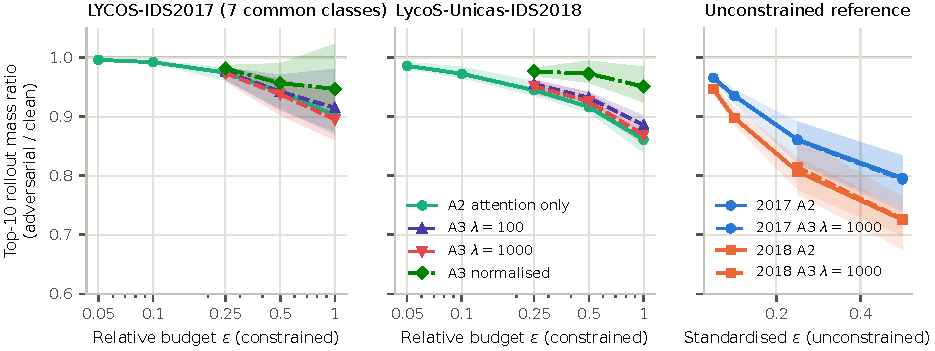
\includegraphics[width=\textwidth]{f_mass_ratio}
  \caption{Top-\paramTopK{} rollout attention mass ratio under A2 and A3, with the unconstrained reference.}
  \label{f_mass_ratio}
\end{figure*}

% Generated by paper_v3/gen/make_tables_v3.py on 2026-10-30. Do not edit.
% Source: results/stage8/sensitivity_stage5.csv
\begin{table}[t]
\centering
\footnotesize
\caption{Attention under protocol-constrained attacks (V1, 7 common classes).}
\label{t_attn_attack}
\begin{tabular}{lcc}
\toprule
Quantity & 2017 & 2018 \\
\midrule
\multicolumn{3}{l}{\textit{Top-10 rollout mass ratio, adversarial / clean (1 = unchanged)}} \\
A2 (attention only), $\epsilon = 0.5$ & $0.946$ {\scriptsize ($0.911$ to $0.967$)} & $0.917$ {\scriptsize ($0.907$ to $0.927$)} \\
A2 (attention only), $\epsilon = 1.0$ & $0.906$ {\scriptsize ($0.864$ to $0.948$)} & $0.861$ {\scriptsize ($0.840$ to $0.874$)} \\
A3 $\lambda{=}1000$ (evasion and attention), $\epsilon = 0.5$ & $0.941$ {\scriptsize ($0.898$ to $0.966$)} & $0.926$ {\scriptsize ($0.917$ to $0.941$)} \\
A3 $\lambda{=}1000$ (evasion and attention), $\epsilon = 1.0$ & $0.900$ {\scriptsize ($0.855$ to $0.947$)} & $0.869$ {\scriptsize ($0.854$ to $0.885$)} \\
A0 (random control), $\epsilon = 1.0$ & $0.994$ {\scriptsize ($0.970$ to $1.025$)} & $0.999$ {\scriptsize ($0.967$ to $1.041$)} \\
A2 unconstrained reference, standardised $\epsilon = 0.5$ & $0.800$ {\scriptsize ($0.748$ to $0.833$)} & $0.726$ {\scriptsize ($0.699$ to $0.743$)} \\
\midrule
\multicolumn{3}{l}{\textit{Evasion success, A1 minus A0}} \\
$\epsilon = 0.5$ & $0.089$ {\scriptsize ($0.002$ to $0.228$)} & $0.082$ {\scriptsize ($-0.004$ to $0.160$)} \\
$\epsilon = 1.0$ & $0.416$ {\scriptsize ($0.216$ to $0.544$)} & $0.416$ {\scriptsize ($0.207$ to $0.550$)} \\
\bottomrule
\end{tabular}
\par\smallskip\parbox{\linewidth}{\scriptsize Macro over the 7 common classes, mean over 3 seeds (seed range). A2 keeps the prediction and minimises the rollout mass on the clean top-10 IG features; A3 also evades. The unconstrained reference has no feature constraints and an $L_\infty$ budget in standardised units, so its budget is not in the units of the constrained attacks. On 2018 no source row is flagged, so V1 equals V0. Other budgets and A3 variants: Appendix~\ref{sec:supp}.}
\end{table}


\paragraph{Faithfulness on flipped rows.}
On rows whose prediction A1 flipped, the margin AOPC gap fell after subtracting the change under A0 for IG, occlusion,
rollout, layer-mean attention, the static class-mean rankings and $|x|$ (Table~\ref{t_flip}).
The change was \flipIGVoneSeventeen{} and \flipIGVoneEighteen{} for IG, \flipOcclVoneSeventeen{} and
\flipOcclVoneEighteen{} for occlusion, \flipRolloutVoneSeventeen{} and \flipRolloutVoneEighteen{} for rollout,
\flipStaticRolloutVoneSeventeen{} and \flipStaticRolloutVoneEighteen{} for the static class-mean rollout, and
\flipAbsXVoneSeventeen{} and \flipAbsXVoneEighteen{} for $|x|$, while the random ranking stayed near zero
(\flipRandomVoneSeventeen{} and \flipRandomVoneEighteen).
The last-layer attention changed with a sign that varied across seeds: \flipLastVoneSeventeen{} on 2017 (seed range
\flipLastVoneSeventeenRange) and \flipLastVoneEighteen{} on 2018 (\flipLastVoneEighteenRange).
On A1 rows that did not flip the change was small for every explainer (IG \notflipIGVoneSeventeen{} and
\notflipIGVoneEighteen), while on rows that the random control A0 flipped to benign by chance (as few as
\nAzeroFlipVoneEighteenMin{} rows in one 2018 seed) the loss was of the same size as on flipped A1 rows on 2017 and
larger on 2018 (IG \azeroflipIGVoneSeventeen{} and \azeroflipIGVoneEighteen).
Because the loss appeared for these explainers on both datasets, including static rankings that the attack cannot
change, was small on rows that did not flip, and appeared also on rows flipped by a random perturbation, it is
consistent with a property of the model at the adversarial point rather than with attack-specific manipulation of
attention; we did not test the mechanism directly.

% Generated by paper_v3/gen/make_tables_v3.py on 2026-10-30. Do not edit.
% Source: results/stage8/flip_split.csv
% Source: results/stage8/flip_split_counts.csv
\begin{table}[t]
\centering
\footnotesize
\setlength{\tabcolsep}{4pt}
\caption{Change of the margin AOPC gap minus the A0 change at $\epsilon = 1$, by row status (V1).}
\label{t_flip}
\sbox0{%
\begin{tabular}{lcccccc}
\toprule
 & \multicolumn{3}{c}{2017} & \multicolumn{3}{c}{2018} \\
Ranking & {\begin{tabular}[t]{@{}c@{}}A1\\flipped\end{tabular}} & {\begin{tabular}[t]{@{}c@{}}A1 not\\flipped\end{tabular}} & {\begin{tabular}[t]{@{}c@{}}A0\\flipped\end{tabular}} & {\begin{tabular}[t]{@{}c@{}}A1\\flipped\end{tabular}} & {\begin{tabular}[t]{@{}c@{}}A1 not\\flipped\end{tabular}} & {\begin{tabular}[t]{@{}c@{}}A0\\flipped\end{tabular}} \\
\midrule
IG & {\begin{tabular}[t]{@{}c@{}}$-11.06$\\{\scriptsize ($-13.04$ to $-9.02$)}\end{tabular}} & {\begin{tabular}[t]{@{}c@{}}$-0.59$\\{\scriptsize ($-2.38$ to $1.17$)}\end{tabular}} & {\begin{tabular}[t]{@{}c@{}}$-11.26$\\{\scriptsize ($-14.08$ to $-7.45$)}\end{tabular}} & {\begin{tabular}[t]{@{}c@{}}$-11.36$\\{\scriptsize ($-12.05$ to $-10.99$)}\end{tabular}} & {\begin{tabular}[t]{@{}c@{}}$-0.46$\\{\scriptsize ($-1.48$ to $0.95$)}\end{tabular}} & {\begin{tabular}[t]{@{}c@{}}$-13.02$\\{\scriptsize ($-14.94$ to $-10.94$)}\end{tabular}} \\
Occlusion & {\begin{tabular}[t]{@{}c@{}}$-12.55$\\{\scriptsize ($-14.26$ to $-10.83$)}\end{tabular}} & {\begin{tabular}[t]{@{}c@{}}$0.43$\\{\scriptsize ($-1.92$ to $3.95$)}\end{tabular}} & {\begin{tabular}[t]{@{}c@{}}$-12.63$\\{\scriptsize ($-15.54$ to $-8.17$)}\end{tabular}} & {\begin{tabular}[t]{@{}c@{}}$-10.61$\\{\scriptsize ($-10.88$ to $-10.25$)}\end{tabular}} & {\begin{tabular}[t]{@{}c@{}}$0.98$\\{\scriptsize ($0.43$ to $1.30$)}\end{tabular}} & {\begin{tabular}[t]{@{}c@{}}$-14.29$\\{\scriptsize ($-16.61$ to $-11.44$)}\end{tabular}} \\
Attn. rollout & {\begin{tabular}[t]{@{}c@{}}$-7.45$\\{\scriptsize ($-8.09$ to $-6.59$)}\end{tabular}} & {\begin{tabular}[t]{@{}c@{}}$0.51$\\{\scriptsize ($-0.58$ to $1.52$)}\end{tabular}} & {\begin{tabular}[t]{@{}c@{}}$-8.35$\\{\scriptsize ($-11.11$ to $-4.49$)}\end{tabular}} & {\begin{tabular}[t]{@{}c@{}}$-7.50$\\{\scriptsize ($-8.93$ to $-5.84$)}\end{tabular}} & {\begin{tabular}[t]{@{}c@{}}$0.27$\\{\scriptsize ($-0.82$ to $1.18$)}\end{tabular}} & {\begin{tabular}[t]{@{}c@{}}$-10.19$\\{\scriptsize ($-13.45$ to $-6.70$)}\end{tabular}} \\
Attn. layer mean & $-7.16$ & $-0.51$ & $-8.95$ & $-7.37$ & $-0.52$ & $-8.30$ \\
Attn. last layer & {\begin{tabular}[t]{@{}c@{}}$1.04$\\{\scriptsize ($-1.33$ to $4.31$)}\end{tabular}} & {\begin{tabular}[t]{@{}c@{}}$0.70$\\{\scriptsize ($-1.94$ to $2.58$)}\end{tabular}} & {\begin{tabular}[t]{@{}c@{}}$0.17$\\{\scriptsize ($-2.54$ to $4.04$)}\end{tabular}} & {\begin{tabular}[t]{@{}c@{}}$-1.16$\\{\scriptsize ($-2.92$ to $0.34$)}\end{tabular}} & {\begin{tabular}[t]{@{}c@{}}$-0.03$\\{\scriptsize ($-0.60$ to $0.84$)}\end{tabular}} & {\begin{tabular}[t]{@{}c@{}}$-1.88$\\{\scriptsize ($-5.26$ to $0.71$)}\end{tabular}} \\
Static rollout (class mean) & $-5.43$ & $0.51$ & $-5.49$ & $-6.19$ & $1.54$ & $-8.41$ \\
Static IG (class mean) & $-9.72$ & $0.33$ & $-9.38$ & $-10.07$ & $0.48$ & $-10.38$ \\
$|x|$ & $-6.60$ & $1.89$ & $-7.00$ & $-5.97$ & $0.87$ & $-7.91$ \\
Random & $0.02$ & $-0.28$ & $-1.19$ & $0.25$ & $-0.30$ & $1.70$ \\
\midrule
Rows per seed & 716, 545, 414 & 185, 356, 487 & 218, 43, 138 & 262, 850, 614 & 723, 135, 371 & 20, 208, 43 \\
\bottomrule
\end{tabular}}%
\ifdim\wd0>\textwidth\resizebox{\textwidth}{!}{\usebox0}\else\usebox0\fi
\par\smallskip\parbox{\linewidth}{\scriptsize Change of the margin AOPC gap from the clean to the adversarial row, minus the mean change over all A0 rows at the same budget; train-mean masking; macro over classes, mean over seeds (seed range for IG, occlusion, rollout and last-layer attention). More negative = larger loss of faithfulness. A0 flipped: rows that the random control flipped to benign by chance. 2017: 7 common classes.}
\end{table}


\subsection{RQ2: consistency monitoring against adaptive attackers}
\label{sec:rq2}
\emph{Answer: the consistency scores helped against an attacker that ignored them, largely without attention, but not
against attackers that optimised the detector's exact score; against those, D$_+$ left more attack rows successful and
undetected than D on both datasets, and the gain measured with a stand-in attacker did not hold.}

\paragraph{Detectors and the non-adaptive attacker.}
Both detectors separated validation positives well (validation AUROC of D \valAurocDSeventeenRange{} on 2017 and
\valAurocDEighteenRange{} on 2018 over seeds, D$_+$ \valAurocDplusSeventeenRange{} and \valAurocDplusEighteenRange;
realised test FPR of D \testFprDSeventeenRange{} and \testFprDEighteenRange).
The validation AUROC is measured on the flipped validation positives that were also used to fit the detectors, so it
is in-sample; the realised test FPR is the out-of-sample figure.
Against A6, which ignores the consistency scores, D$_+$ detected more of the evading rows than D: the paired TPR
difference D$_+$ minus D on A6 rows ($\lambda = 1$) was \tprAsixOneVoneSeventeen{} (\tprAsixOneVoneSeventeenCI) on 2017
and \tprAsixOneVoneEighteen{} (\tprAsixOneVoneEighteenCI) on 2018 (Table~\ref{t_attacks}).

% Generated by paper_v3/gen/make_tables_v3.py on 2026-10-30. Do not edit.
% Source: results/stage8/sensitivity_defenders.csv
% Source: results/stage8/sensitivity_paired.csv
% Source: results/stage9/a8x/summary_tpr.csv
% Source: results/stage9/a8x/summary_extra.csv
\begin{table}[t]
\centering
\footnotesize
\setlength{\tabcolsep}{4pt}
\caption{Success and undetected share per attack at $\epsilon = 1$ (V1, 7 common classes), and the paired TPR difference D$_+$ minus D on the flipped rows of each attack.}
\label{t_attacks}
\textit{2017}\par\smallskip
\sbox0{%
\begin{tabular}{lllcccc}
\toprule
Attack & Aimed at & Attacker & Success & Undet. D & Undet. D$_+$ & TPR D$_+$ minus D [95\% CI] \\
\midrule
A1 & none &  & $0.620$ {\scriptsize ($0.459$ to $0.795$)} & $0.016$ {\scriptsize ($0.000$ to $0.046$)} & $0.001$ {\scriptsize ($0.000$ to $0.003$)} & $+0.023$ {\scriptsize [$+0.016$, $+0.031$]} \\
A6 $\lambda{=}1$ & D & exact & $0.496$ {\scriptsize ($0.275$ to $0.714$)} & $0.204$ {\scriptsize ($0.148$ to $0.272$)} & $0.086$ {\scriptsize ($0.009$ to $0.210$)} & $+0.238$ {\scriptsize [$+0.213$, $+0.265$]} \\
A6 $\lambda{=}100$ & D & exact & $0.319$ {\scriptsize ($0.108$ to $0.489$)} & $0.127$ {\scriptsize ($0.007$ to $0.234$)} & $0.052$ {\scriptsize ($0.001$ to $0.132$)} & $+0.234$ {\scriptsize [$+0.199$, $+0.271$]} \\
A6 norm. & D & exact & $0.613$ {\scriptsize ($0.535$ to $0.735$)} & $0.181$ {\scriptsize ($0.098$ to $0.307$)} & $0.055$ {\scriptsize ($0.006$ to $0.135$)} & $+0.204$ {\scriptsize [$+0.185$, $+0.223$]} \\
A8 $\lambda{=}1$ & D$_+$ & stand-in & $0.524$ {\scriptsize ($0.332$ to $0.740$)} & $0.162$ {\scriptsize ($0.134$ to $0.191$)} & $0.141$ {\scriptsize ($0.064$ to $0.277$)} & $+0.040$ {\scriptsize [$+0.013$, $+0.066$]} \\
A8 $\lambda{=}100$ & D$_+$ & stand-in & $0.427$ {\scriptsize ($0.213$ to $0.637$)} & $0.117$ {\scriptsize ($0.024$ to $0.178$)} & $0.125$ {\scriptsize ($0.012$ to $0.279$)} & $-0.017$ {\scriptsize [$-0.049$, $+0.013$]} \\
A8 norm. & D$_+$ & stand-in & $0.620$ {\scriptsize ($0.508$ to $0.776$)} & $0.120$ {\scriptsize ($0.069$ to $0.182$)} & $0.112$ {\scriptsize ($0.037$ to $0.262$)} & $+0.013$ {\scriptsize [$-0.010$, $+0.034$]} \\
A8x $\lambda{=}1$ & D$_+$ & exact obj. & $0.519$ {\scriptsize ($0.307$ to $0.747$)} & $0.191$ {\scriptsize ($0.125$ to $0.294$)} & $0.282$ {\scriptsize ($0.097$ to $0.436$)} & $-0.175$ {\scriptsize [$-0.203$, $-0.148$]} \\
A8x $\lambda{=}100$ & D$_+$ & exact obj. & $0.438$ {\scriptsize ($0.253$ to $0.640$)} & $0.162$ {\scriptsize ($0.038$ to $0.320$)} & $0.242$ {\scriptsize ($0.020$ to $0.438$)} & $-0.182$ {\scriptsize [$-0.210$, $-0.154$]} \\
A8x norm. & D$_+$ & exact obj. & $0.621$ {\scriptsize ($0.497$ to $0.774$)} & $0.175$ {\scriptsize ($0.081$ to $0.287$)} & $0.252$ {\scriptsize ($0.051$ to $0.477$)} & $-0.124$ {\scriptsize [$-0.150$, $-0.097$]} \\
\bottomrule
\end{tabular}}%
\ifdim\wd0>\textwidth\resizebox{\textwidth}{!}{\usebox0}\else\usebox0\fi
\par\medskip
\textit{2018}\par\smallskip
\sbox0{%
\begin{tabular}{lllcccc}
\toprule
Attack & Aimed at & Attacker & Success & Undet. D & Undet. D$_+$ & TPR D$_+$ minus D [95\% CI] \\
\midrule
A1 & none &  & $0.584$ {\scriptsize ($0.266$ to $0.863$)} & $0.001$ {\scriptsize ($0.000$ to $0.001$)} & $0.000$ {\scriptsize ($0.000$ to $0.001$)} & $+0.001$ {\scriptsize [$-0.001$, $+0.002$]} \\
A6 $\lambda{=}1$ & D & exact & $0.303$ {\scriptsize ($0.129$ to $0.504$)} & $0.014$ {\scriptsize ($0.002$ to $0.036$)} & $0.002$ {\scriptsize ($0.000$ to $0.007$)} & $+0.037$ {\scriptsize [$+0.021$, $+0.051$]} \\
A6 $\lambda{=}100$ & D & exact & $0.280$ {\scriptsize ($0.092$ to $0.481$)} & $0.006$ {\scriptsize ($0.001$ to $0.014$)} & $0.003$ {\scriptsize ($0.000$ to $0.008$)} & $+0.013$ {\scriptsize [$+0.001$, $+0.025$]} \\
A6 norm. & D & exact & $0.493$ {\scriptsize ($0.281$ to $0.722$)} & $0.013$ {\scriptsize ($0.001$ to $0.025$)} & $0.000$ {\scriptsize ($0.000$ to $0.001$)} & $+0.025$ {\scriptsize [$+0.018$, $+0.033$]} \\
A8 $\lambda{=}1$ & D$_+$ & stand-in & $0.335$ {\scriptsize ($0.123$ to $0.602$)} & $0.007$ {\scriptsize ($0.001$ to $0.016$)} & $0.013$ {\scriptsize ($0.001$ to $0.020$)} & $-0.017$ {\scriptsize [$-0.032$, $-0.003$]} \\
A8 $\lambda{=}100$ & D$_+$ & stand-in & $0.324$ {\scriptsize ($0.131$ to $0.552$)} & $0.007$ {\scriptsize ($0.000$ to $0.019$)} & $0.013$ {\scriptsize ($0.001$ to $0.018$)} & $-0.016$ {\scriptsize [$-0.031$, $+0.001$]} \\
A8 norm. & D$_+$ & stand-in & $0.504$ {\scriptsize ($0.237$ to $0.748$)} & $0.000$ {\scriptsize ($0.000$ to $0.001$)} & $0.006$ {\scriptsize ($0.000$ to $0.011$)} & $-0.012$ {\scriptsize [$-0.018$, $-0.006$]} \\
A8x $\lambda{=}1$ & D$_+$ & exact obj. & $0.336$ {\scriptsize ($0.136$ to $0.572$)} & $0.009$ {\scriptsize ($0.000$ to $0.021$)} & $0.021$ {\scriptsize ($0.001$ to $0.045$)} & $-0.037$ {\scriptsize [$-0.055$, $-0.019$]} \\
A8x $\lambda{=}100$ & D$_+$ & exact obj. & $0.317$ {\scriptsize ($0.124$ to $0.522$)} & $0.008$ {\scriptsize ($0.000$ to $0.021$)} & $0.019$ {\scriptsize ($0.000$ to $0.045$)} & $-0.032$ {\scriptsize [$-0.050$, $-0.015$]} \\
A8x norm. & D$_+$ & exact obj. & $0.515$ {\scriptsize ($0.268$ to $0.734$)} & $0.012$ {\scriptsize ($0.000$ to $0.021$)} & $0.016$ {\scriptsize ($0.000$ to $0.027$)} & $-0.009$ {\scriptsize [$-0.021$, $+0.003$]} \\
\bottomrule
\end{tabular}}%
\ifdim\wd0>\textwidth\resizebox{\textwidth}{!}{\usebox0}\else\usebox0\fi
\par\smallskip\parbox{\linewidth}{\scriptsize Success: share of source rows predicted benign; Undet.: also below the detector threshold at 5\% FPR on validation benign rows. Mean over seeds pooled over rows (seed range). TPR difference: paired bootstrap over the flipped rows (1,000 draws). Attacker: exact, the attacker's objective is the exact detector score; stand-in, differentiable stand-ins for the consistency scores; exact obj., the exact score with surrogate gradients for the eight rank-based scores. The rows of an attack aimed at D$_+$ were optimised against D$_+$, so a negative TPR difference on them is expected by construction; the equal-effort comparison is Table~\ref{t_union_adaptive}.}
\end{table}


The controls (Section~\ref{sec:detectors}, Table~\ref{t_dplus_ablation}) show that this gain against A6 is largely
obtained without attention: the TPR difference to D was \ablBMinusDSeventeen{} and \ablBMinusDEighteen{} for the
attribution-only control b and \ablCtwoMinusDSeventeen{} and \ablCtwoMinusDEighteen{} for c2 with logit and distance
statistics, while c0 (\ablCzeroMinusDSeventeen) and c1 (\ablConeMinusDSeventeen) show that the regulariser and the
number of scores do not explain it.
Shuffled attention from another row of the same class (a1) kept most of the gain on 2017 and all of it on 2018
(\ablAoneMinusDSeventeen{} and \ablAoneMinusDEighteen), attention from clean benign rows (a2) kept
\ablAtwoMinusDSeventeen{} and \ablAtwoMinusDEighteen, and the pairing of a row's own attention with its attribution,
D$_+$ minus a1 against A6, added \ablPairSeventeen{} (\ablPairSeventeenCI) on 2017 and nothing detectable on 2018
(\ablPairEighteen, \ablPairEighteenCI).

% Generated by paper/make_tables_v2.py on 2026-10-30. Do not edit.
% Source: results/stage9/ablation/summary_detection.csv
% Source: results/stage9/ablation/summary_paired.csv
% Source: results/stage9/ablation/summary_defenders.csv
\begin{table}[t]
\centering
\footnotesize
\caption{Controls for D$_+$: detection of A1 and A6 rows by D, D$_+$ and the six controls (V1, $\epsilon = 1$).}
\label{t_dplus_ablation}
\textit{2017 (1{,}675 A1 rows, 1{,}341 A6 $\lambda{=}1$ rows)}\par\smallskip
\sbox0{%
\begin{tabular}{lcccccccc}
\toprule
Quantity & D & D$_+$ & a1 & a2 & b & c0 & c1 & c2 \\
\midrule
TPR on A1 & $0.975$ & $0.998$ & $0.996$ & $0.980$ & $0.998$ & $0.975$ & $0.976$ & $0.994$ \\
TPR on A6 $\lambda{=}1$ & $0.589$ & $0.827$ & $0.782$ & $0.688$ & $0.855$ & $0.589$ & $0.547$ & $0.782$ \\
A6 $\lambda{=}1$ minus D &  & {\begin{tabular}[t]{@{}c@{}}$0.238$\\{\scriptsize [$0.214$, $0.265$]}\end{tabular}} & {\begin{tabular}[t]{@{}c@{}}$0.192$\\{\scriptsize [$0.166$, $0.217$]}\end{tabular}} & {\begin{tabular}[t]{@{}c@{}}$0.099$\\{\scriptsize [$0.075$, $0.125$]}\end{tabular}} & {\begin{tabular}[t]{@{}c@{}}$0.265$\\{\scriptsize [$0.238$, $0.294$]}\end{tabular}} & {\begin{tabular}[t]{@{}c@{}}$0.000$\\{\scriptsize [$0.000$, $0.000$]}\end{tabular}} & {\begin{tabular}[t]{@{}c@{}}$-0.043$\\{\scriptsize [$-0.055$, $-0.029$]}\end{tabular}} & {\begin{tabular}[t]{@{}c@{}}$0.193$\\{\scriptsize [$0.172$, $0.216$]}\end{tabular}} \\
D$_+$ minus control &  &  & {\begin{tabular}[t]{@{}c@{}}$0.045$\\{\scriptsize [$0.028$, $0.065$]}\end{tabular}} & {\begin{tabular}[t]{@{}c@{}}$0.139$\\{\scriptsize [$0.113$, $0.166$]}\end{tabular}} & {\begin{tabular}[t]{@{}c@{}}$-0.028$\\{\scriptsize [$-0.050$, $-0.002$]}\end{tabular}} & {\begin{tabular}[t]{@{}c@{}}$0.238$\\{\scriptsize [$0.212$, $0.264$]}\end{tabular}} & {\begin{tabular}[t]{@{}c@{}}$0.280$\\{\scriptsize [$0.254$, $0.305$]}\end{tabular}} & {\begin{tabular}[t]{@{}c@{}}$0.045$\\{\scriptsize [$0.015$, $0.075$]}\end{tabular}} \\
Realised test FPR & $0.052$ & $0.053$ & $0.060$ & $0.057$ & $0.056$ & $0.052$ & $0.053$ & $0.050$ \\
\bottomrule
\end{tabular}}%
\ifdim\wd0>\textwidth\resizebox{\textwidth}{!}{\usebox0}\else\usebox0\fi
\par\medskip
\textit{2018 (1{,}726 A1 rows, 896 A6 $\lambda{=}1$ rows)}\par\smallskip
\sbox0{%
\begin{tabular}{lcccccccc}
\toprule
Quantity & D & D$_+$ & a1 & a2 & b & c0 & c1 & c2 \\
\midrule
TPR on A1 & $0.999$ & $0.999$ & $0.998$ & $0.999$ & $1.000$ & $0.999$ & $0.998$ & $1.000$ \\
TPR on A6 $\lambda{=}1$ & $0.955$ & $0.992$ & $0.991$ & $0.975$ & $0.997$ & $0.960$ & $0.954$ & $0.993$ \\
A6 $\lambda{=}1$ minus D &  & {\begin{tabular}[t]{@{}c@{}}$0.037$\\{\scriptsize [$0.022$, $0.051$]}\end{tabular}} & {\begin{tabular}[t]{@{}c@{}}$0.036$\\{\scriptsize [$0.023$, $0.049$]}\end{tabular}} & {\begin{tabular}[t]{@{}c@{}}$0.020$\\{\scriptsize [$0.010$, $0.030$]}\end{tabular}} & {\begin{tabular}[t]{@{}c@{}}$0.041$\\{\scriptsize [$0.028$, $0.055$]}\end{tabular}} & {\begin{tabular}[t]{@{}c@{}}$0.004$\\{\scriptsize [$0.001$, $0.009$]}\end{tabular}} & {\begin{tabular}[t]{@{}c@{}}$-0.001$\\{\scriptsize [$-0.008$, $0.006$]}\end{tabular}} & {\begin{tabular}[t]{@{}c@{}}$0.038$\\{\scriptsize [$0.025$, $0.052$]}\end{tabular}} \\
D$_+$ minus control &  &  & {\begin{tabular}[t]{@{}c@{}}$0.001$\\{\scriptsize [$-0.007$, $0.010$]}\end{tabular}} & {\begin{tabular}[t]{@{}c@{}}$0.017$\\{\scriptsize [$0.006$, $0.028$]}\end{tabular}} & {\begin{tabular}[t]{@{}c@{}}$-0.004$\\{\scriptsize [$-0.012$, $0.002$]}\end{tabular}} & {\begin{tabular}[t]{@{}c@{}}$0.032$\\{\scriptsize [$0.019$, $0.047$]}\end{tabular}} & {\begin{tabular}[t]{@{}c@{}}$0.038$\\{\scriptsize [$0.023$, $0.055$]}\end{tabular}} & {\begin{tabular}[t]{@{}c@{}}$-0.001$\\{\scriptsize [$-0.009$, $0.008$]}\end{tabular}} \\
Realised test FPR & $0.055$ & $0.049$ & $0.055$ & $0.058$ & $0.048$ & $0.055$ & $0.052$ & $0.055$ \\
\bottomrule
\end{tabular}}%
\ifdim\wd0>\textwidth\resizebox{\textwidth}{!}{\usebox0}\else\usebox0\fi
\par\smallskip\parbox{\linewidth}{\scriptsize Controls (Section~\ref{sec:methods}): a1, attention of another row of the same true class; a2, attention of clean benign validation rows; b, occlusion and GradientSHAP instead of attention; c0, D with the regularisation of D$_+$; c1, D with 12 noise features; c2, D with 12 logit and distance statistics. Thresholds at 5\% FPR on validation benign rows. TPR on the source rows that the attack flipped to benign, pooled over seeds 0 to 2; differences are paired TPR differences with a 95\% paired bootstrap interval (1,000 draws over the flipped rows pooled over seeds, threshold-centred per seed), computed separately from the intervals in Section~\ref{sec:sens}, so the interval of D$_+$ minus D can differ from them in the last digit. Realised test FPR: mean over seeds on the benign test negatives.}
\end{table}


\paragraph{Attackers that model the consistency scores.}
Against A8, which models the consistency scores through stand-ins, the gain largely disappeared: the paired TPR
difference on A8 rows ($\lambda = 1$) was \tprAeightOneVoneSeventeen{} (\tprAeightOneVoneSeventeenCI) on 2017 and
\tprAeightOneVoneEighteen{} (\tprAeightOneVoneEighteenCI) on 2018.
Against A8x, which optimises the exact score of D$_+$ (Section~\ref{sec:attacks}), D$_+$ detected fewer of the attack
rows than D: \xtprAxOneVoneSeventeen{} (\xtprAxOneVoneSeventeenCI) on 2017 and \xtprAxOneVoneEighteen{}
(\xtprAxOneVoneEighteenCI) on 2018, and from \xtprAxVoneRangeSeventeen{} over the three settings on 2017
(Table~\ref{t_attacks}).
A8x flipped about as many rows as A8 (success \xsuccAxOneVoneSeventeen{} against \xsuccAeightOneVoneSeventeen{} on 2017)
but left more of them undetected by D$_+$ (\xundetAxOneVoneSeventeen{} against \xundetAeightOneVoneSeventeen).
These rows were optimised against D$_+$, so this comparison alone is not evidence; the equal-effort union is.

\paragraph{Equal-effort comparison.}
Under equal attacker effort (Table~\ref{t_union_adaptive}, Figure~\ref{f_headline}), with D facing A1 and A6 and D$_+$
facing A1 and A8x, D$_+$ left more source rows successful and undetected than D: \axHeadVoneSeventeenDplus{} against
\axHeadVoneSeventeenD{} on 2017, a difference of \axHeadVoneSeventeen{} (\paramCILevel{} CI \axHeadVoneSeventeenCI),
and \axHeadVoneEighteenDplus{} against \axHeadVoneEighteenD{} on 2018, a difference of \axHeadVoneEighteen{}
(\axHeadVoneEighteenCI).
With A8 instead of A8x the 2017 difference had been \axStandinVoneSeventeen{} (\axStandinVoneSeventeenCI), and on 2018
\axStandinVoneEighteen{} (\axStandinVoneEighteenCI).
Per seed, the 2017 differences were \axHeadVoneSeventeenSeeds{} and the 2018 differences \axHeadVoneEighteenSeeds{}
(seeds 0, 1 and 2); \axHeadOppSeedsSeventeen{} seed on 2017 and \axHeadOppSeedsEighteen{} on 2018 had the opposite
sign.
By the outcome rule recorded before the A8x runs (Section~\ref{sec:protocol}), the 2017 gain of D$_+$ against A8 did
not hold against the exact-objective attacker.

These numbers come with caveats that limit how far they generalise.
They rest on \nSeeds{} seeds, and on each dataset \axHeadOppSeedsSeventeen{} seed (2017) and
\axHeadOppSeedsEighteen{} seed (2018) had the opposite sign; the interval is a bootstrap over source rows within seed
and does not capture variation between seeds.
A8x still uses surrogate gradients for the \nRankScores{} rank-based scores; a better search on these terms could only
find further undetected rows for D$_+$.
The controls a1 and a2 faced stand-in attackers, so their comparison with D$_+$ under A8x is not at equal attacker
strength, and control b was not attacked adaptively because its run exceeded the memory of the graphics card.
On 2018 D alone left only \axHeadVoneEighteenD{} of the source rows undetected, so the 2018 difference sits near a floor
and its lower bound is close to $0$.
Finally, the equal-effort protocol fixes candidates, steps and settings, not optimiser quality: whether A6 is as strong
an attack on D as A8x is on D$_+$ was not measured (see below and Section~\ref{sec:limitations}).

\begin{figure*}[t]
  \centering
  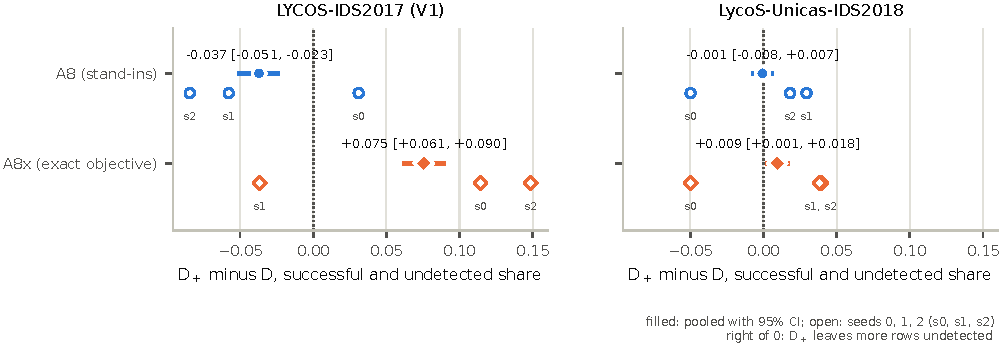
\includegraphics[width=\textwidth]{f_headline}
  \caption{Equal-effort union at $\epsilon = \paramEpsHead$ (V1): D$_+$ minus D in the share of successful and
    undetected source rows when D$_+$ faces the stand-in attacker A8 or the exact-objective attacker A8x (D faces A6 in
    both). Filled marks: pooled difference with the \paramCILevel{} paired bootstrap interval (within seed); open
    marks: seeds 0, 1 and 2.}
  \label{f_headline}
\end{figure*}

% Generated by paper_v3/gen/make_tables_v3.py on 2026-10-30. Do not edit.
% Source: results/stage9/a8x/summary_union.csv
% Source: results/stage9/a6x/summary_union.csv
% Source: results/stage9/adaptive/summary_union.csv
% Source: results/stage9/a8x/summary_extra.csv
% Source: results/stage9/adaptive/{2017,2018}/standin_quality.csv
\begin{table}[t]
\centering
\footnotesize
\setlength{\tabcolsep}{3pt}
\caption{Equal-effort union at $\epsilon = 1$ (V1): share of source rows that are successful and undetected, each detector against its own attackers.}
\label{t_union_adaptive}
\textit{2017, V1 (901 source rows per seed)}\par\smallskip
\sbox0{%
\begin{tabular}{lllcccc}
\toprule
Detector & Attacker & Type & Undet. & Minus D [95\% CI] & Seeds 0 / 1 / 2 & Minus D$_+$ (A8x) [95\% CI] \\
\midrule
D & A1 + A6 $\times 3$ & exact & $0.266$ & (reference) &  & $-0.075$ {\scriptsize [$-0.090$, $-0.061$]} \\
D & A1 + A6x $\times 3$ & exact & $0.266$ & $0.000$ {\scriptsize [$+0.000$, $+0.000$]} & $0.000\,/\,0.000\,/\,0.000$ &  \\
\textbf{D$_+$} & \textbf{A1 + A8x $\times 3$} & exact obj. & $0.341$ & \textbf{$+0.075$ {\scriptsize [$+0.061$, $+0.090$]}} & $+0.114\,/\,-0.037\,/\,+0.149$ & (reference) \\
D$_+$ & A1 + A8 $\times 3$ & stand-in & $0.229$ & $-0.037$ {\scriptsize [$-0.051$, $-0.023$]} & $+0.031\,/\,-0.058\,/\,-0.084$ &  \\
\midrule
c0 & A1 + own $\times 3$ & exact & $0.266$ & $0.000$ {\scriptsize [$-0.007$, $+0.009$]} & $-0.004\,/\,+0.002\,/\,+0.003$ & $-0.075$ {\scriptsize [$-0.089$, $-0.061$]} \\
c1 & A1 + own $\times 3$ & exact & $0.280$ & $+0.014$ {\scriptsize [$+0.004$, $+0.024$]} & $+0.011\,/\,-0.001\,/\,+0.032$ & $-0.061$ {\scriptsize [$-0.075$, $-0.048$]} \\
c2 & A1 + own $\times 3$ & exact & $0.273$ & $+0.008$ {\scriptsize [$-0.006$, $+0.023$]} & $-0.075\,/\,+0.081\,/\,+0.018$ & $-0.068$ {\scriptsize [$-0.083$, $-0.052$]} \\
a1 & A1 + own $\times 3$ & stand-in ($R^2$ $0.983$ / $0.800$) & $0.344$ & $+0.078$ {\scriptsize [$+0.063$, $+0.094$]} & $+0.206\,/\,-0.112\,/\,+0.141$ & $+0.003$ {\scriptsize [$-0.010$, $+0.017$]} \\
a2 & A1 + own $\times 3$ & stand-in ($R^2$ $0.980$ / $0.803$) & $0.278$ & $+0.013$ {\scriptsize [$-0.003$, $+0.029$]} & $-0.031\,/\,-0.032\,/\,+0.101$ & $-0.063$ {\scriptsize [$-0.075$, $-0.050$]} \\
b & \multicolumn{6}{l}{not attacked adaptively (Section~\ref{sec:limitations})} \\
\bottomrule
\end{tabular}}%
\ifdim\wd0>\textwidth\resizebox{\textwidth}{!}{\usebox0}\else\usebox0\fi
\par\medskip
\textit{2018, V1 (985 source rows per seed)}\par\smallskip
\sbox0{%
\begin{tabular}{lllcccc}
\toprule
Detector & Attacker & Type & Undet. & Minus D [95\% CI] & Seeds 0 / 1 / 2 & Minus D$_+$ (A8x) [95\% CI] \\
\midrule
D & A1 + A6 $\times 3$ & exact & $0.023$ & (reference) &  & $-0.009$ {\scriptsize [$-0.018$, $-0.001$]} \\
D & A1 + A6x $\times 3$ & exact & $0.023$ & $0.000$ {\scriptsize [$+0.000$, $+0.000$]} & $0.000\,/\,0.000\,/\,0.000$ &  \\
\textbf{D$_+$} & \textbf{A1 + A8x $\times 3$} & exact obj. & $0.032$ & \textbf{$+0.009$ {\scriptsize [$+0.001$, $+0.018$]}} & $-0.050\,/\,+0.040\,/\,+0.039$ & (reference) \\
D$_+$ & A1 + A8 $\times 3$ & stand-in & $0.022$ & $-0.001$ {\scriptsize [$-0.008$, $+0.007$]} & $-0.050\,/\,+0.029\,/\,+0.018$ &  \\
\midrule
c0 & A1 + own $\times 3$ & exact & $0.015$ & $-0.008$ {\scriptsize [$-0.013$, $-0.004$]} & $-0.009\,/\,0.000\,/\,-0.015$ & $-0.018$ {\scriptsize [$-0.025$, $-0.010$]} \\
c1 & A1 + own $\times 3$ & exact & $0.019$ & $-0.004$ {\scriptsize [$-0.008$, $+0.001$]} & $-0.006\,/\,+0.010\,/\,-0.015$ & $-0.013$ {\scriptsize [$-0.020$, $-0.006$]} \\
c2 & A1 + own $\times 3$ & exact & $0.055$ & $+0.032$ {\scriptsize [$+0.023$, $+0.042$]} & $-0.049\,/\,+0.161\,/\,-0.015$ & $+0.023$ {\scriptsize [$+0.013$, $+0.032$]} \\
a1 & A1 + own $\times 3$ & stand-in ($R^2$ $0.946$ / $0.726$) & $0.006$ & $-0.016$ {\scriptsize [$-0.022$, $-0.011$]} & $-0.040\,/\,+0.006\,/\,-0.015$ & $-0.026$ {\scriptsize [$-0.032$, $-0.019$]} \\
a2 & A1 + own $\times 3$ & stand-in ($R^2$ $0.947$ / $0.736$) & $0.021$ & $-0.001$ {\scriptsize [$-0.007$, $+0.004$]} & $-0.010\,/\,+0.020\,/\,-0.014$ & $-0.011$ {\scriptsize [$-0.018$, $-0.004$]} \\
b & \multicolumn{6}{l}{not attacked adaptively (Section~\ref{sec:limitations})} \\
\bottomrule
\end{tabular}}%
\ifdim\wd0>\textwidth\resizebox{\textwidth}{!}{\usebox0}\else\usebox0\fi
\par\smallskip\parbox{\linewidth}{\scriptsize A source row counts if any candidate aimed at that detector flips it to benign and stays below the detector's threshold (5\% FPR). Minus D: difference to D under A1 + A6 $\times 3$ (for the A6x row: D under A6x minus D under A6); a positive value means more rows evade undetected, which is worse for the defender. Paired bootstrap over source rows within seed, 1,000 draws; the interval does not capture variation between seeds. Type: exact, the attacker optimises the exact score; exact obj., the exact score with surrogate gradients for the eight rank-based consistency scores; stand-in, differentiable stand-ins ($R^2$ median / minimum over features and seeds). Comparisons of a1 or a2 with D$_+$ under A8x are not at equal attacker strength. The D$_+$ row with A8 is shown for comparison only.}
\end{table}


On 2017 the direction held per attack setting (\axLamOneVoneSeventeen, \axLamHundredVoneSeventeen{} and
\axNormVoneSeventeen; Table~\ref{t_a8x_setting}) and on the other row sets (Section~\ref{sec:rq3}), and the paired TPR
difference on A8x rows was negative for every setting and row set (largest value \xtprAxMaxSeventeen;
Table~\ref{t_a8x_tpr}).

\paragraph{Selection rule (A6x).}
\label{sec:a6x}
A8x keeps the iterate with the lowest true D$_+$ score, while A6 keeps its own rule, so part of the reversal could have
come from the selection rather than from the consistency scores.
A6x gives the attacker of D the selection rule of A8x.
It kept a different iterate in \sxRowsDiffer{} of \sxRowsAll{} attacked rows, but changed the flipped status of
\sxFlipChanged{} rows and the undetected status of \sxUndetChanged{} rows, because A6 already ranks iterates that are
flipped and below the threshold under the exact score of D first.
D's undetected share under A1 and A6x therefore equalled that under A1 and A6 in every seed and row set (largest
absolute difference \sxSelMaxAbs), and the 2017 difference D$_+$ minus D kept a lower bound of \sxHeadVoneSeventeenLo{}
(\sxHeadVoneSeventeenCI, separate bootstrap draws).
By the rule recorded before the A6x runs, the reversal does not come from the selection rule.

Whether A8x is simply a stronger optimiser than A6 is a different question.
The A8x rows were not aimed at D, yet D left a similar share of them undetected as of the A6 rows aimed at it (2017,
share of source rows: \evadeDAxOneSeventeen{} against \evadeDAsixOneSeventeen{} for $\lambda = 1$,
\evadeDAxHundredSeventeen{} against \evadeDAsixHundredSeventeen{} for $\lambda = 100$); the remaining differences between
the two attackers concern scores that D does not have, so the relative optimiser strength remains unmeasured.

\paragraph{Controls under their own adaptive attackers.}
\nControlsAttacked{} of the \nControlsAll{} controls were attacked by adversaries that modelled their own scores
(Table~\ref{t_union_adaptive}).
Against D, the controls with exact attackers stayed close to D on 2017 (c0 \cmdCzeroVoneSeventeen{},
\cmdCzeroVoneSeventeenCI; c1 \cmdConeVoneSeventeen{}, \cmdConeVoneSeventeenCI; c2 \cmdCtwoVoneSeventeen{},
\cmdCtwoVoneSeventeenCI), while a1 left more rows undetected (\cmdAoneVoneSeventeen{}, \cmdAoneVoneSeventeenCI); on
2018, c0 (\cmdCzeroVoneEighteen) and a1 (\cmdAoneVoneEighteen) left fewer rows undetected than D and c2 more
(\cmdCtwoVoneEighteen).
No control left clearly fewer rows undetected than D on both datasets.
Against D$_+$ under A8x, every control except a1 on 2017 and c2 on 2018 left fewer rows undetected (2017: c0
\cmxCzeroVoneSeventeen, c1 \cmxConeVoneSeventeen, c2 \cmxCtwoVoneSeventeen, a1 \cmxAoneVoneSeventeen{}
\cmxAoneVoneSeventeenCI, a2 \cmxAtwoVoneSeventeen; 2018: c2 \cmxCtwoVoneEighteen{} \cmxCtwoVoneEighteenCI).
For c0, c1 and c2 this comparison is at roughly equal attacker strength (exact against exact apart from the surrogate
ranks of A8x; their attackers keep the selection rule of A6, which A6x showed to be equivalent for D but which was not
tested for them).
For a1 and a2 it is not: their attackers used stand-ins (median $R^2$ \rtwoMedAoneSeventeen{} and
\rtwoMedAtwoSeventeen{} on 2017), so their shares may be too low, as A8's were for D$_+$.
The comparisons with D$_+$ under A8 are in Table~\ref{t_union_a8}.
On these two datasets, consistency monitoring did not make the confidence-and-distance detector harder to evade for an
attacker that optimised its exact score.

\subsection{RQ3: dataset dependence and near duplicates}
\label{sec:rq3}
\emph{Answer: the level of successful and undetected rows depended strongly on the dataset and was dominated by one
class on each; the sign of D$_+$ minus D under A8x was the same on both datasets, its size was not; removing near
duplicates changed no conclusion.}

\paragraph{Dataset dependence.}
Detector strength differed strongly between the datasets.
Under A6 with $\lambda = 1$, the share of source rows that evaded D undetected was \undetDAsixOneVoneSeventeen{}
(\undetDAsixOneVoneSeventeenRange) on 2017 and \undetDAsixOneVoneEighteen{} (\undetDAsixOneVoneEighteenRange) on 2018
(Table~\ref{t_attacks}), and under the equal-effort union \axHeadVoneSeventeenD{} and \axHeadVoneEighteenD.
On 2018, \pcTopClassEighteen{} was the only class with a non-trivial share (\pcTopEighteen; every other class at most
\pcRestMaxEighteen), while on 2017 \pcTopClassSeventeen{} dominated (\pcTopSeventeen; every other class at most
\pcRestMaxSeventeen; Table~\ref{t_per_class_v1}).
Under A8x against D$_+$, DDoS again dominated on 2018, while on 2017 SSH-Patator joined Bot, with a seed range that
spans almost the whole scale (Table~\ref{t_per_class_v1}).
The difference between the datasets in detector strength was much larger than the difference between D and D$_+$:
the sign of D$_+$ minus D under A8x was the same on both datasets, its size was not (\axHeadVoneSeventeen{} and
\axHeadVoneEighteen).

% Generated by paper_v3/gen/make_tables_v3.py on 2026-10-30. Do not edit.
% Source: results/stage8/sensitivity_per_class.csv
% Source: results/stage9/a8x/{2017,2018}/seed*/rows_A8x_lam1.parquet
% Source: src/stage9_dplus_ablation.py keep_pos (V1 rows)
\begin{table}[t]
\centering
\footnotesize
\setlength{\tabcolsep}{4pt}
\caption{Per-class share of successful and undetected source rows at $\epsilon = 1$ (V1): A6 $\lambda{=}1$ against D and A8x $\lambda{=}1$ against D$_+$.}
\label{t_per_class_v1}
\sbox0{%
\begin{tabular}{lcccccc}
\toprule
 & \multicolumn{3}{c}{2017} & \multicolumn{3}{c}{2018} \\
Class & A6 vs D & A8x vs D$_+$ & n & A6 vs D & A8x vs D$_+$ & n \\
\midrule
Bot & {\begin{tabular}[t]{@{}c@{}}$0.824$\\{\scriptsize ($0.611$ to $0.944$)}\end{tabular}} & {\begin{tabular}[t]{@{}c@{}}$0.764$\\{\scriptsize ($0.590$ to $0.931$)}\end{tabular}} & 144 & {\begin{tabular}[t]{@{}c@{}}$0.000$\\{\scriptsize ($0.000$ to $0.000$)}\end{tabular}} & {\begin{tabular}[t]{@{}c@{}}$0.000$\\{\scriptsize ($0.000$ to $0.000$)}\end{tabular}} & 150 \\
DDoS & {\begin{tabular}[t]{@{}c@{}}$0.000$\\{\scriptsize ($0.000$ to $0.000$)}\end{tabular}} & {\begin{tabular}[t]{@{}c@{}}$0.000$\\{\scriptsize ($0.000$ to $0.000$)}\end{tabular}} & 150 & {\begin{tabular}[t]{@{}c@{}}$0.080$\\{\scriptsize ($0.000$ to $0.233$)}\end{tabular}} & {\begin{tabular}[t]{@{}c@{}}$0.124$\\{\scriptsize ($0.007$ to $0.280$)}\end{tabular}} & 150 \\
DoS GoldenEye & {\begin{tabular}[t]{@{}c@{}}$0.078$\\{\scriptsize ($0.000$ to $0.227$)}\end{tabular}} & {\begin{tabular}[t]{@{}c@{}}$0.127$\\{\scriptsize ($0.007$ to $0.367$)}\end{tabular}} & 150 & {\begin{tabular}[t]{@{}c@{}}$0.000$\\{\scriptsize ($0.000$ to $0.000$)}\end{tabular}} & {\begin{tabular}[t]{@{}c@{}}$0.000$\\{\scriptsize ($0.000$ to $0.000$)}\end{tabular}} & 150 \\
DoS Hulk & {\begin{tabular}[t]{@{}c@{}}$0.067$\\{\scriptsize ($0.000$ to $0.161$)}\end{tabular}} & {\begin{tabular}[t]{@{}c@{}}$0.054$\\{\scriptsize ($0.000$ to $0.148$)}\end{tabular}} & 149 & {\begin{tabular}[t]{@{}c@{}}$0.000$\\{\scriptsize ($0.000$ to $0.000$)}\end{tabular}} & {\begin{tabular}[t]{@{}c@{}}$0.011$\\{\scriptsize ($0.000$ to $0.033$)}\end{tabular}} & 150 \\
DoS Slowloris & {\begin{tabular}[t]{@{}c@{}}$0.000$\\{\scriptsize ($0.000$ to $0.000$)}\end{tabular}} & {\begin{tabular}[t]{@{}c@{}}$0.000$\\{\scriptsize ($0.000$ to $0.000$)}\end{tabular}} & 77$^\ast$ & {\begin{tabular}[t]{@{}c@{}}$0.002$\\{\scriptsize ($0.000$ to $0.007$)}\end{tabular}} & {\begin{tabular}[t]{@{}c@{}}$0.000$\\{\scriptsize ($0.000$ to $0.000$)}\end{tabular}} & 150 \\
SSH-Patator & {\begin{tabular}[t]{@{}c@{}}$0.187$\\{\scriptsize ($0.000$ to $0.487$)}\end{tabular}} & {\begin{tabular}[t]{@{}c@{}}$0.651$\\{\scriptsize ($0.000$ to $0.987$)}\end{tabular}} & 150 & {\begin{tabular}[t]{@{}c@{}}$0.004$\\{\scriptsize ($0.000$ to $0.013$)}\end{tabular}} & {\begin{tabular}[t]{@{}c@{}}$0.000$\\{\scriptsize ($0.000$ to $0.000$)}\end{tabular}} & 150 \\
Web attack & {\begin{tabular}[t]{@{}c@{}}$0.189$\\{\scriptsize ($0.000$ to $0.321$)}\end{tabular}} & {\begin{tabular}[t]{@{}c@{}}$0.239$\\{\scriptsize ($0.012$ to $0.420$)}\end{tabular}} & 81$^\ast$ & {\begin{tabular}[t]{@{}c@{}}$0.004$\\{\scriptsize ($0.000$ to $0.012$)}\end{tabular}} & {\begin{tabular}[t]{@{}c@{}}$0.008$\\{\scriptsize ($0.000$ to $0.024$)}\end{tabular}} & 85$^\ast$ \\
\bottomrule
\end{tabular}}%
\ifdim\wd0>\textwidth\resizebox{\textwidth}{!}{\usebox0}\else\usebox0\fi
\par\smallskip\parbox{\linewidth}{\scriptsize Mean over seeds pooled over rows (seed range). n: V1 source rows per seed; $^\ast$ marks n < 100. Single attacks, not the union. All source rows (V0) with A8 in Appendix~\ref{sec:supp}.}
\end{table}


\paragraph{Near duplicates.}
Test rows with a near duplicate in the training set were common in both datasets (\ndAllSeventeen{} and
\ndAllEighteen{} of all test rows) and concentrated in DoS Slowloris and, on 2017, web attack (Section~\ref{sec:setup}).
On 2017, flagged rows were easier for both detectors: on A6 rows ($\lambda = 1$) the TPR of D was \tprDNdSeventeen{} on
flagged and \tprDOtherSeventeen{} on other source rows, and the FPR of D was \fprDNdSeventeen{} on flagged and
\fprDOtherSeventeen{} on other benign test negatives (Appendix~\ref{sec:sens}).
Moving from V0 to V1 and V2 (Table~\ref{t_neardup_compact}) changed the attention mass ratio under A2 and A3 by at
most \sensMaxMassChange{} and the faithfulness loss on flipped rows for IG and rollout by at most \sensMaxFlipChange{}
(absolute values from the unrounded means over seeds, both datasets).
The 2017 equal-effort difference under A8x was \axHeadVzeroSeventeen{}, \axHeadVoneSeventeen{} and
\axHeadVtwoSeventeen{} on V0, V1 and V2, and on 2018, where V1 equals V0, \axHeadVoneEighteen{} and
\axHeadVtwoEighteen{} (\axHeadVtwoEighteenCI) on V2.
With the stand-in attacker A8 the 2017 difference changed more with the row set (\axStandinVzeroSeventeen,
\axStandinVoneSeventeen, \axStandinVtwoSeventeen).

% Generated by paper_v3/gen/make_tables_v3.py on 2026-10-30. Do not edit.
% Source: results/stage8/sensitivity_stage5.csv
% Source: results/stage8/sensitivity_defenders.csv
% Source: results/stage8/sensitivity_paired.csv
% Source: results/stage9/a8x/summary_union.csv
% Source: results/stage9/a8x/summary_tpr.csv
\begin{table}[t]
\centering
\footnotesize
\setlength{\tabcolsep}{4pt}
\caption{Near-duplicate sensitivity of the headline quantities: all source rows (V0), near duplicates removed (V1, primary), DoS Slowloris and web attack removed (V2).}
\label{t_neardup_compact}
\sbox0{%
\begin{tabular}{lcccccc}
\toprule
 & \multicolumn{3}{c}{2017} & \multicolumn{3}{c}{2018} \\
Quantity & V0 & V1 & V2 & V0 & V1 & V2 \\
\midrule
A2 mass ratio, $\epsilon = 1$ & $0.902$ & $0.906$ & $0.927$ & $0.861$ & $0.861$ & $0.866$ \\
Flipped A1, AOPC gap minus A0, IG & $-10.70$ & $-11.06$ & $-10.73$ & $-11.36$ & $-11.36$ & $-11.09$ \\
Flipped A1, AOPC gap minus A0, rollout & $-7.61$ & $-7.45$ & $-6.73$ & $-7.50$ & $-7.50$ & $-6.74$ \\
Undet.\ D, A6 $\lambda{=}1$ & $0.185$ & $0.204$ & $0.226$ & $0.014$ & $0.014$ & $0.017$ \\
TPR D$_+$ minus D, A6 $\lambda{=}1$ rows & $+0.199$ & $+0.238$ & $+0.271$ & $+0.037$ & $+0.037$ & $+0.048$ \\
TPR D$_+$ minus D, A8x $\lambda{=}1$ rows & $-0.146$ & $-0.175$ & $-0.194$ & $-0.037$ & $-0.037$ & $-0.052$ \\
Union D$_+$ (A8x) minus D & {\begin{tabular}[t]{@{}c@{}}$+0.080$\\{\scriptsize [$+0.066$, $+0.093$]}\end{tabular}} & {\begin{tabular}[t]{@{}c@{}}$+0.075$\\{\scriptsize [$+0.061$, $+0.090$]}\end{tabular}} & {\begin{tabular}[t]{@{}c@{}}$+0.070$\\{\scriptsize [$+0.053$, $+0.086$]}\end{tabular}} & {\begin{tabular}[t]{@{}c@{}}$+0.009$\\{\scriptsize [$+0.001$, $+0.018$]}\end{tabular}} & {\begin{tabular}[t]{@{}c@{}}$+0.009$\\{\scriptsize [$+0.001$, $+0.018$]}\end{tabular}} & {\begin{tabular}[t]{@{}c@{}}$+0.012$\\{\scriptsize [$+0.001$, $+0.023$]}\end{tabular}} \\
Union D$_+$ (A8, stand-in) minus D & {\begin{tabular}[t]{@{}c@{}}$-0.025$\\{\scriptsize [$-0.039$, $-0.012$]}\end{tabular}} & {\begin{tabular}[t]{@{}c@{}}$-0.037$\\{\scriptsize [$-0.051$, $-0.023$]}\end{tabular}} & {\begin{tabular}[t]{@{}c@{}}$-0.049$\\{\scriptsize [$-0.064$, $-0.032$]}\end{tabular}} & {\begin{tabular}[t]{@{}c@{}}$-0.001$\\{\scriptsize [$-0.008$, $+0.006$]}\end{tabular}} & {\begin{tabular}[t]{@{}c@{}}$-0.001$\\{\scriptsize [$-0.008$, $+0.007$]}\end{tabular}} & {\begin{tabular}[t]{@{}c@{}}$0.000$\\{\scriptsize [$-0.011$, $+0.009$]}\end{tabular}} \\
\bottomrule
\end{tabular}}%
\ifdim\wd0>\textwidth\resizebox{\textwidth}{!}{\usebox0}\else\usebox0\fi
\par\smallskip\parbox{\linewidth}{\scriptsize Means over seeds (attacks) or pooled over rows (detectors); union with the paired bootstrap 95\% CI. Rows are filtered after the fact; models, attacks and detectors are unchanged. On 2018 no source row is flagged, so V1 equals V0. Full tables in Appendix~\ref{sec:sens}.}
\end{table}

